\documentclass{article}
\usepackage[font=small, labelfont=bf]{caption}
\usepackage{sectsty}
\usepackage{dblfloatfix} 
\usepackage{fixltx2e}
\usepackage{graphicx}
\usepackage{color}
\usepackage[letterpaper, margin=0.75in]{geometry}
\usepackage{amsmath}
\usepackage{amsfonts}
\usepackage{tikz}
\usepackage{pgfplots}
\usepackage{parskip}
\usepackage{multicol}
\usepackage{wrapfig}
\usepackage[compact]{titlesec}
\usepackage{float}
\usepackage{pdfpages}
\usepackage{euler}

\begin{document}
\graphicspath{ {Images/} }
\sectionfont{\fontsize{11}{0}\selectfont}
\setlength{\headsep}{0pt}

\titlespacing{\section}{0pt}{*0}{*0}
\titlespacing{\subsection}{0pt}{*0}{*0}
\titlespacing{\subsubsection}{0pt}{*0}{*0}

\setlength{\parindent}{0pt}

\title{Algorithmic Biosynthesis: Staged Glycan Assembly}
\author{Anjali Jaiman and Mukund Thattai}
\maketitle



\begin{figure*}
    \includegraphics[width=\textwidth]{Figure_1.pdf}
	\caption{A) O-glycosylation mainly takes place in the Golgi apparatus. Proteins from the ER are shipped to the Golgi apparatus, where they are glycosylated before they are transported to the plasma membrane.  B) Locally acting enzymes. B) A glycan is an oligosaccharide. A GalNac monosaccharide is covalently attached to a serine or threonine residue on a glycoprotein. Each monosaccharide ring has multiple carbons that can bind to other monosaccharides. This allows glycans to branch. C) In the Golgi apparatus GTases transfer a single donor monosaccharide from a nucleotide sugar onto an acceptor monosaccharide on the growing glycan. Most GTases have a minimal specificity of donor, acceptor and carbon pair linkages. D) Some GTases common to mammals [see Supplemental Figure 1 for full reaction network]}
\end{figure*}  

\begin{figure*}
    \includegraphics[width=\textwidth]{Figure_2.pdf}
	\caption{A) Sources of diversity: Incompleteness B) Sources of diversity: Competition. C) Sources of diversity: Polymerization.}
\end{figure*}

\begin{figure*}[h]
    \includegraphics[width=\textwidth]{Figure_3.pdf}
	\caption{A)Entropy as a function of residence time comparing a cyclic reaction network (blue), a cyclic reaction network with a competing tip (red) and a totally ordered reaction network (orange). B) Entropy as a function of average residence time comparing a totally ordered reaction network (orange), a partially ordered reaction network (light blue), and totally ordered reaction network with competition (green).}
\end{figure*}


\begin{figure}[h]
    \includegraphics[width=0.5\textwidth]{Figure_4.pdf}
	\caption{A) Distribution of glycosylation products formed by putting all required locally acting enzymes in each of the three compartments. B) Distribution of glycosylation products when the required enzymes are compartmentalized according to a ``best" partition. C) Distribution of glycosylation products when the average residence times in each compartment of the ``best" partition are not taken as equal. Instead, they are taken 1:5:5. In blue, gillespe simulations were run with total average time is taken at 96.3 for each of the three programs. In mirrored plot (green), the three simulations were run with total average time at 4.8.D) Compares the KL divergences of the three programs above as the distance between a uniform distribution of the four structures and the program distribution as a function of average residence time.}
\end{figure}


\begin{figure*}[t]
    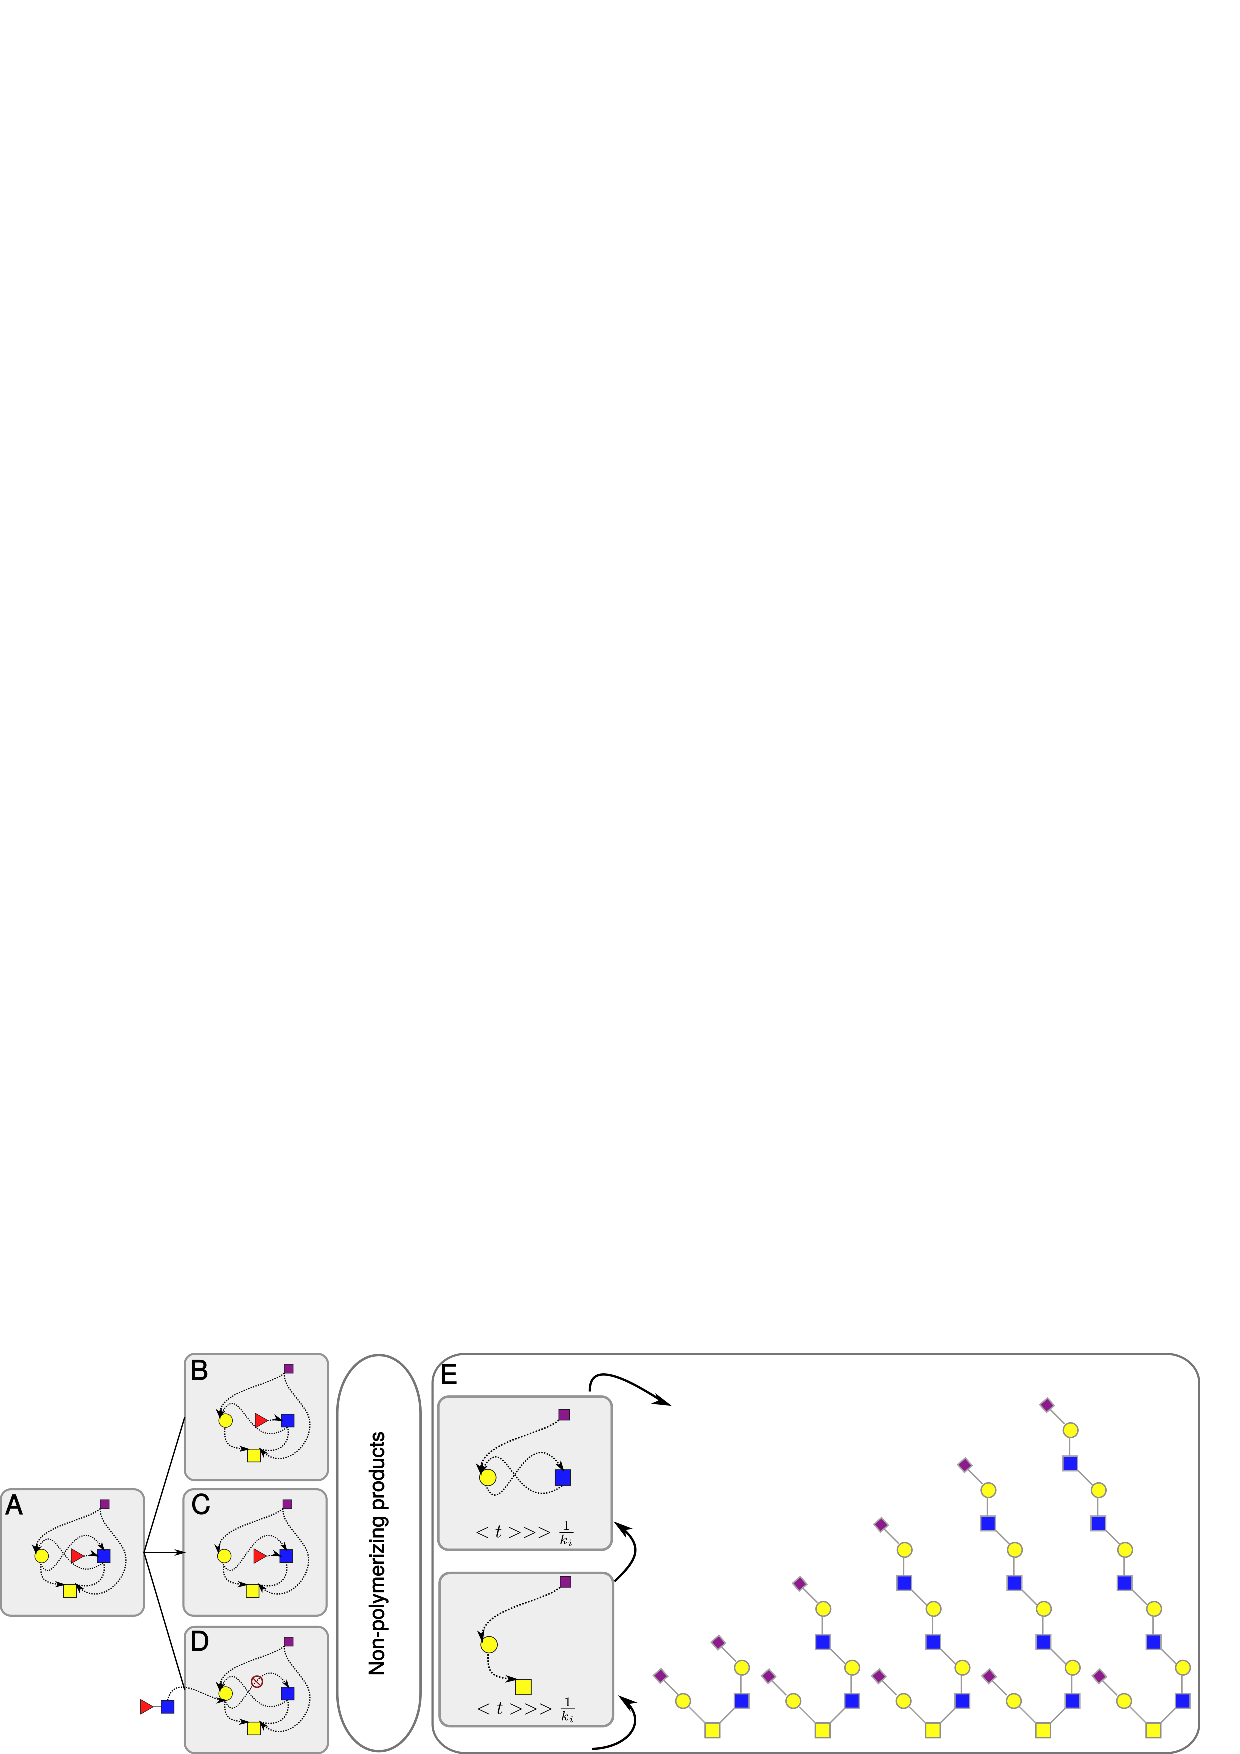
\includegraphics[width=\textwidth]{Figure_6.pdf}
	\caption{A) O-glycans found on equine chorionic gonadotropin \cite{Hokke1994}. O-glycans found on a recombinant MUC1 expressed in B) T47D, C) MDA-MB231, D)ZR-75-1 human breast adenocarcinoma cell lines \cite{Muller2002}. All structure sets contain one or more of the glycan structures found in hCG o-glycan set described above and contain a subset of the linkages found. They are ordered left to right (or top to bottom) in terms of greatest to lowest yields. Trace amounts of other species reported by \cite{Muller2002} were not included.}
\end{figure*}


\begin{figure}
\includegraphics[width=\textwidth]{SuppFig_1.pdf}
\end{figure}

\begin{figure}
\includegraphics[width=\textwidth]{SuppFig_3.pdf}
\end{figure}





\end{document}